\documentclass[12pt, a4paper]{article}
\usepackage[a4paper, left=2cm, right=2cm, top=3cm, bottom=3cm]{geometry}

\usepackage[english]{babel}
\usepackage[utf8]{inputenc}
\usepackage{fancyhdr}

\usepackage{enumitem}
\usepackage{amsmath}
\usepackage{mathtools}

\usepackage{tikz}
\usetikzlibrary{arrows.meta,shapes.multipart}

\pagestyle{fancy}
\fancyhf{}
\lhead{Operations Research}
\chead{Blatt 03}
\rhead{Til Mohr, 405959}

\begin{document}

\section*{Aufgabe 19}
Wir modellieren das Problem als kürzeste Wege Problem in einem gewichteten, gerichteten Graphen $G=(V,E), c$ mit:
\begin{itemize}
	\item $V \coloneqq \{Jan, Feb, Mar, Apr, May, Jun, Jul, Aug, Sep, Oct, Nov, Dec\} \cup \{End\}$, wobei hier der Knoten $End$ das Ende des Jahres darstellen soll.
	\item $E \widehat{=}$ Aufträge, also: \\
		  $E \coloneqq \{(i,j) \vert i,j \in V, i \neq j,$ Es existiert ein Auftrag, welcher im Monat $i$ beginnt, und im Monat $j$ bzw. $End$ endet.$\} \cup \{(i, j) \vert $Monat $j$ folgt auf Monat $i\} \cup \{(Dec, End)\}$
	\item $c_{(i,j)} = \begin{cases}
							-p,&(i,j) \text{ ist einem Auftag zugeordnet mit Profit p}\\
							0,& \text{sonst}
					   \end{cases}$
\end{itemize}

Das Beispiel aus der Aufgabenstellung liefert also folgenden Graphen:\\
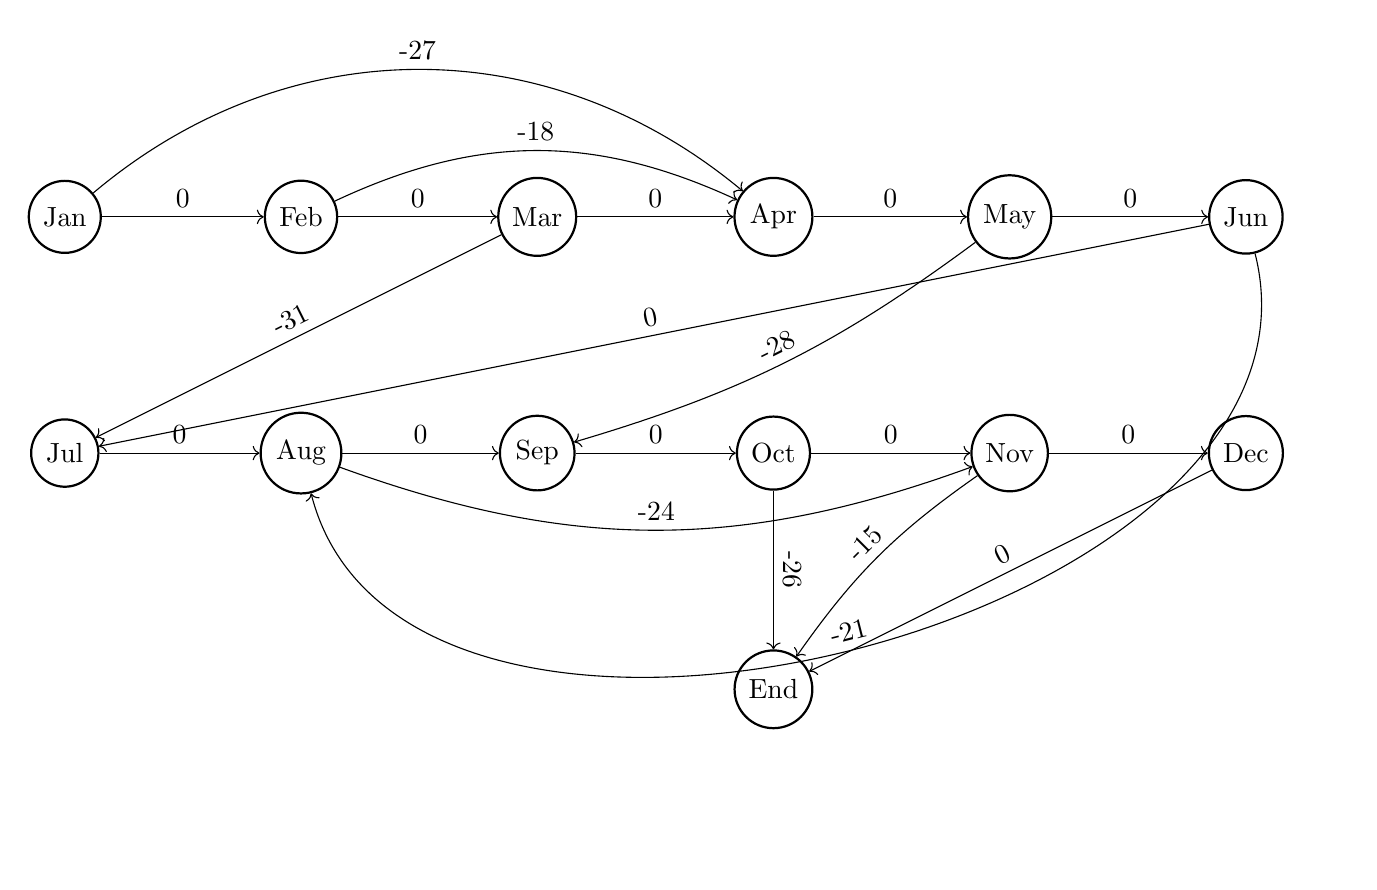
\begin{tikzpicture}[every node/.style={circle,thick,draw,align=center}, node distance=3cm]
	\node (Jan) {Jan};
	\node[right of=Jan] (Feb) {Feb};
	\node[right of=Feb] (Mar) {Mar};
	\node[right of=Mar] (Apr) {Apr};
	\node[right of=Apr] (May) {May};
	\node[right of=May] (Jun) {Jun};
	\node[below of=Jan] (Jul) {Jul};
	\node[right of=Jul] (Aug) {Aug};
	\node[right of=Aug] (Sep) {Sep};
	\node[right of=Sep] (Oct) {Oct};
	\node[right of=Oct] (Nov) {Nov};
	\node[right of=Nov] (Dec) {Dec};
	\node[below of=Oct] (End) {End};
	
	\path[->,every node/.style={sloped,anchor=south,auto=false}]
		(Jan) edge node {0} (Feb)
		(Feb) edge node {0} (Mar)
		(Mar) edge node {0} (Apr)
		(Apr) edge node {0} (May)
		(May) edge node {0} (Jun)
		(Jun) edge node {0} (Jul)
		(Jul) edge node {0} (Aug)
		(Aug) edge node {0} (Sep)
		(Sep) edge node {0} (Oct)
		(Oct) edge node {0} (Nov)
		(Nov) edge node {0} (Dec)
		(Dec) edge node {0} (End)
		
		(Jan) edge[bend left=40] node {-27} (Apr)
		(Feb) edge[bend left=25] node {-18} (Apr)
		(Mar) edge[bend left=0] node {-31} (Jul)
		(May) edge[bend left=10] node {-28} (Sep)
		(Jun) edge[bend left=90] node {-21} (Aug)
		(Aug) edge[bend right=20] node {-24} (Nov)
		(Oct) edge[bend left=0] node {-26} (End)
		(Nov) edge[bend right=10] node {-15} (End)
	;
\end{tikzpicture}

Eine zulässige Lösung des kürzeste Wege Problems auf $G$ von $Jan$ nach $End$ entspricht also einer optimalen Wahl der Aufträge in diesem Jahr.\\
Der Graph $G$ ist immer zusammenhängend und sogar azyklisch, folglich gibt es immer einen kürzesten Weg von $Jan$ nach $End$. Wählt man keinen Auftrag aus, so führt der Weg durch alle Knoten und hat eine Länge von $0$. Mit jedem angenommenen Auftrag verkürzt sich der Weg in Anbetracht auf besuchte Knoten und Länge (verkürzt sich immer um den Profit von dem Auftrag).\\

Somit ist also die optimale Auswahl von Aufträgen immer die, mit welchen den Aufträgen zugeordneten Kanten der kürzeste Weg in $G$ existiert.

\end{document}